\documentclass{beamer}
\usepackage[utf8]{inputenc}
\usepackage{eurosym}

\graphicspath{{src/}}


%Information to be included in the title page:
\title{Using Random Fourier Features with Random Forests}
\author{Albert Ribes}
\institute{UPC --- FIB}
\date{April 9, 2018}


\usetheme{Madrid}
% \usecolortheme{beaver}



\begin{document}





\frame{\titlepage}

\begin{frame}
\frametitle{Context}

% 
\includegraphics[height=3.5cm]{machine_learning}
% 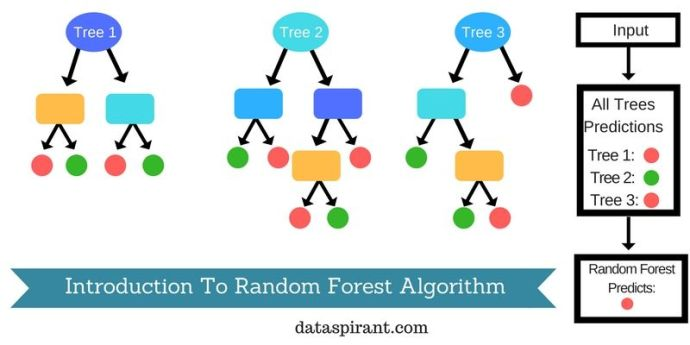
\includegraphics[height=3.5cm]{random_forest}


\includegraphics[width=0.45\textwidth]{machine_learning}%
\hfill
% 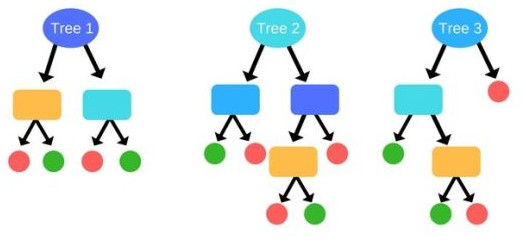
\includegraphics[width=0.45\textwidth]{random_forest_3}

\includegraphics[width=4cm]{brain}
\end{frame}

\begin{frame}
\frametitle{Context}
\framesubtitle{Random Forest}

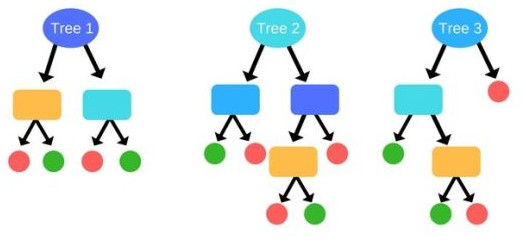
\includegraphics[width=\textwidth]{random_forest_3}

\end{frame}

\begin{frame}
\frametitle{Context}
\framesubtitle{Random Fourier Features}

\begin{center}
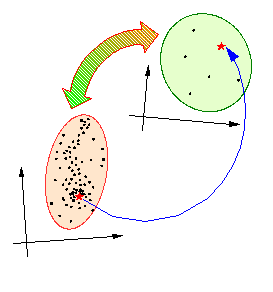
\includegraphics[scale=0.7]{space_mapping_2}
% 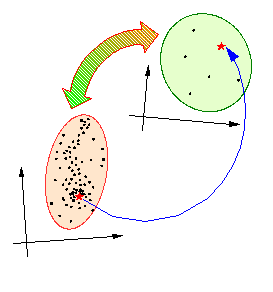
\includegraphics[totalheight=\textheight,keepaspectratio]{space_mapping_2}
\end{center}


\end{frame}


\begin{frame}
\frametitle{Scope}

\begin{block}{One mapping per forest}
First generate one mapping and then use original Random Forest algorithm with the new data
\end{block}

\only<1>{\begin{block}{One mapping per tree}
Generate one mapping for each of the trees, and build and train them with the original tree-building algorithm
\end{block}}

\only<2>{\begin{exampleblock}{One mapping per tree}
Generate one mapping for each of the trees, and build and train them with the original tree-building algorithm
\end{exampleblock}}

\begin{block}{One mapping per node}
Generate a mapping in each split step during the tree building
\end{block}


\end{frame}
%
%
% \begin{frame}
% \frametitle{Scope}
%
% \begin{block}{One mapping per forest}
% First generate one mapping and then use original Random Forest algorithm with the new data
% \end{block}
%
% % \begin{block}{One mapping per tree}
% % Generate one mapping for each of the trees, and build and train them with the original tree-building algorithm
% % \end{block}
%
% \begin{exampleblock}{One mapping per tree}
% Generate one mapping for each of the trees, and build and train them with the original tree-building algorithm
% \end{exampleblock}
%
% \begin{block}{One mapping per node}
% Generate a mapping in each split step during the tree building
% \end{block}
%
%
% \end{frame}


\begin{frame}
\frametitle{Planning}

\begin{block}{Theoretical Approach}
\begin{itemize}
    \item Study Random Forest Algorithm
    \item Study Random Fourier Features Mapping
    \item Study the way to mix them
\end{itemize}
\end{block}

\begin{block}{Algorithm Implementation}
\begin{itemize}
    \item Code for the mapping
    \item Modifications to the Random Forest Algorithm
\end{itemize}
\end{block}

\begin{block}{Testing}
\begin{itemize}
    \item Time and accuracy tests
\end{itemize}
\end{block}

\end{frame}

\begin{frame}
\frametitle{Planning}
\framesubtitle{Workflow}
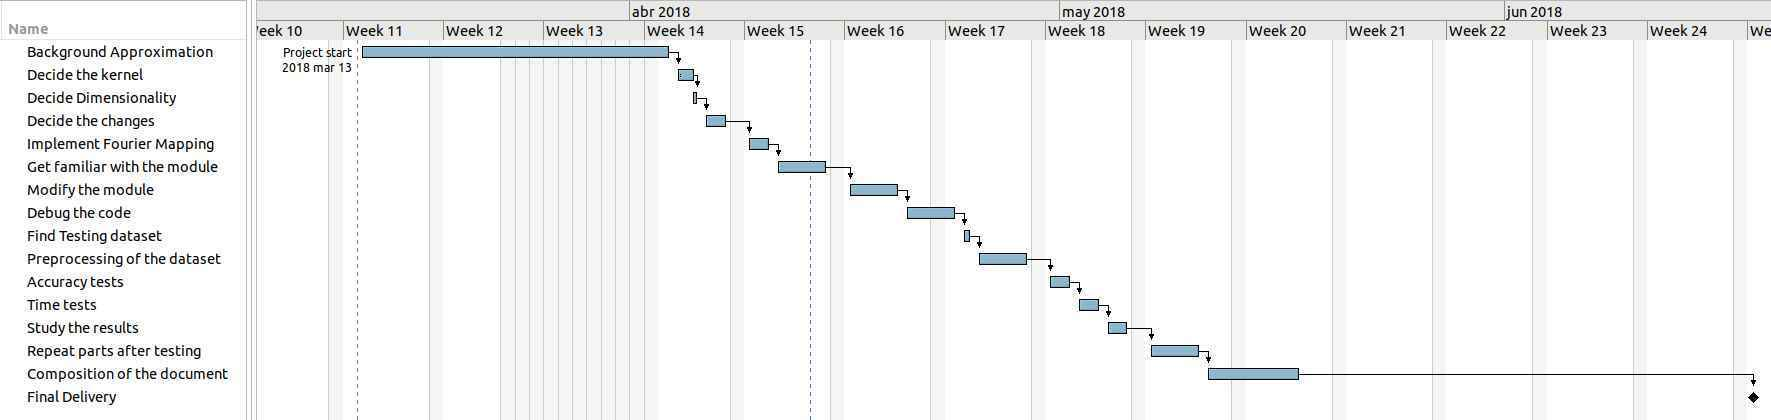
\includegraphics[width=\textwidth]{gantt2}
\end{frame}

% \begin{frame}
% \frametitle{Planning}
% \framesubtitle{Algorithm Implementation}
% Texto
% \end{frame}

% \begin{frame}
% \frametitle{Planning}
% \framesubtitle{Testing}
% Texto
% \end{frame}

\begin{frame}
\frametitle{Budget}

\begin{block}{Roles}
\begin{itemize}
    \item Expert in Machine Learning
    \item Programmer
    \item Tester
\end{itemize}
\end{block}
\begin{itemize}
    \item Labour cost: \(240 \text{ hours of work} \cdot \frac{30 \text{ \euro}}{1 \text{ hour}} = 7200 \text{ \euro}\)
    \item Indirect Costs: Transport (150 \euro)
    \item Depreciation: Laptop (25.6 \euro)
\end{itemize}

\begin{block}{Total cost}
    7375.6 \euro
\end{block}
\end{frame}


\begin{frame}
\frametitle{Sustainability}
\begin{center}
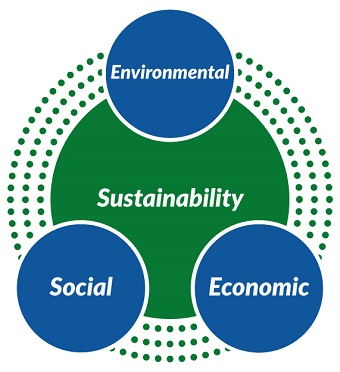
\includegraphics[width=0.45\textwidth]{sustan}
\end{center}

\end{frame}








\end{document}
